% Terremoto
\newpage
%\thispagestyle{empty}
\begin{recipe}[source={Internet},
	portion={1 porción},
	preparationtime={\unit[1]{Minuto}}
	]{Terremoto}
%	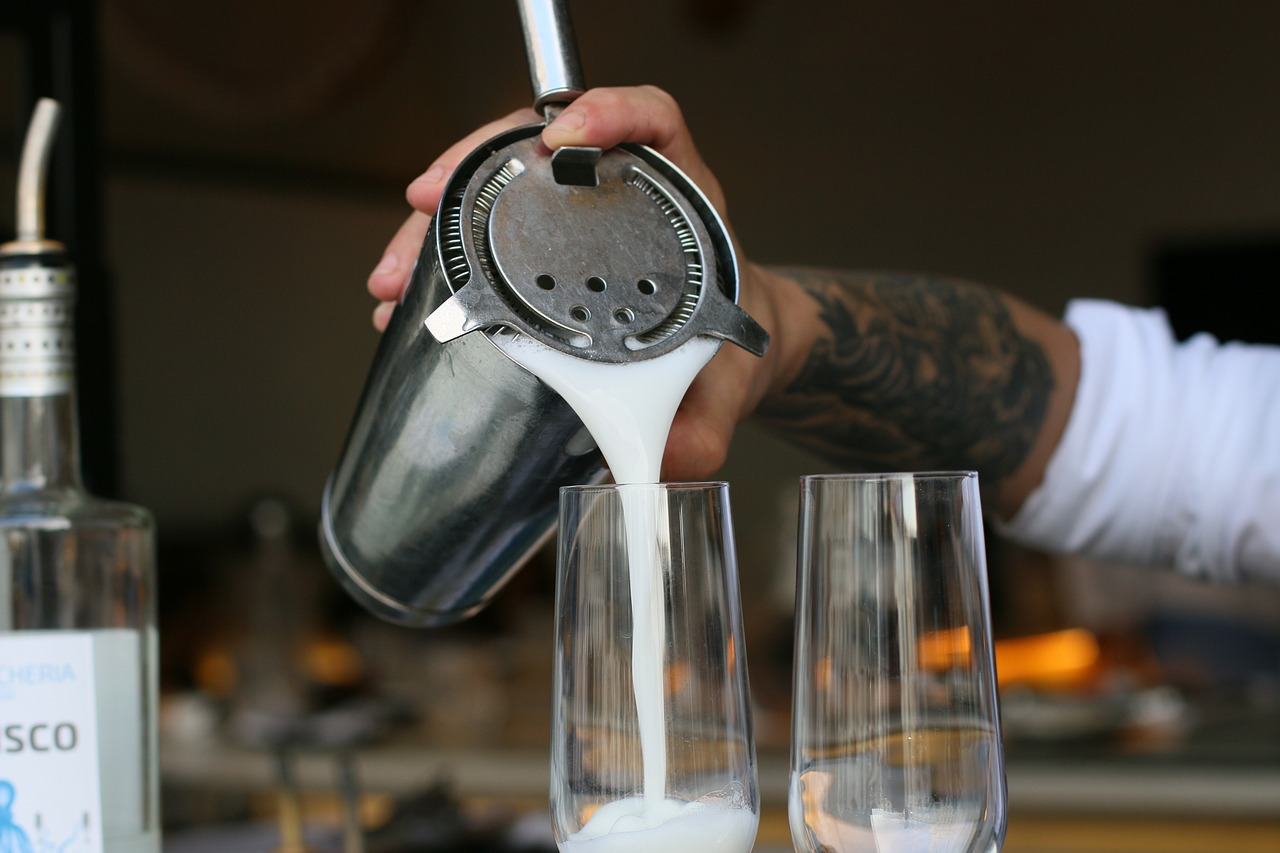
\includegraphics[width=0.25\textwidth]{pisco-sour}
	\introduction{
		Esta receta la vi por internet. Específicamente en un canal de Insta...
	}
	\ingredients{
		30 & \unit[ml] granadina \\
		3 & Cucharadas soperas de helado de piña \\
		& Pipeño 
	}
	\preparation{
		\begin{enumerate}
			\item Verter todo en un vaso, revolver por aproximadamente 10 segundos.
			\item Servir.
		\end{enumerate}
	}
%	\hint{
%		
%	}
\end{recipe}